\section{Durchführung}
Als erstes wurden die drei Messzylinder gewogen. Anschließend wurden die Messzylinder mit 80\ ml $KOH$ gefüllt. Die gefüllten Messzylinder wurden gewogen, um den Volumenfehler des Messzylinders zu umgehen. Danach wurde das Dreikammer-Elektrolysegefäß mit der $KOH$- Lösung gefüllt. Anschließend wurden die Platin-Elektroden angebracht. Der Strom wurde angeschaltet. Während der Dauer von 90\ min wurde versucht die Stromstärke konstant auf 50\ mA zu halten. Währendessen wurde am Amfang jede Minute und ab 15\ min alle 5\ min die Stromstärke protokollliert. Zur Messung der Stromstärke wurde das Multimeter  Voltkraft M4660M verwendet, gemessen wurde auf der Einstellung 200\ mA. Außerdem wurden dreimal je 10\ ml $KOH$ zur kontrolle gegentitriert mit 0.1\ M $HCL$. Nach einer Messdauer von 90 Minuten wurde das Dreikammer-Elektrolysegefäß geleert. Anschließend wurde die $KOH$-Lösung ein letztes mal in den Messzylindern, die zum befüllen benutzt wurden, gewogen. Danach wurden zweimal 10\ ml  aus jeder Kammer titriert.
\begin{figure}[H]
\centering
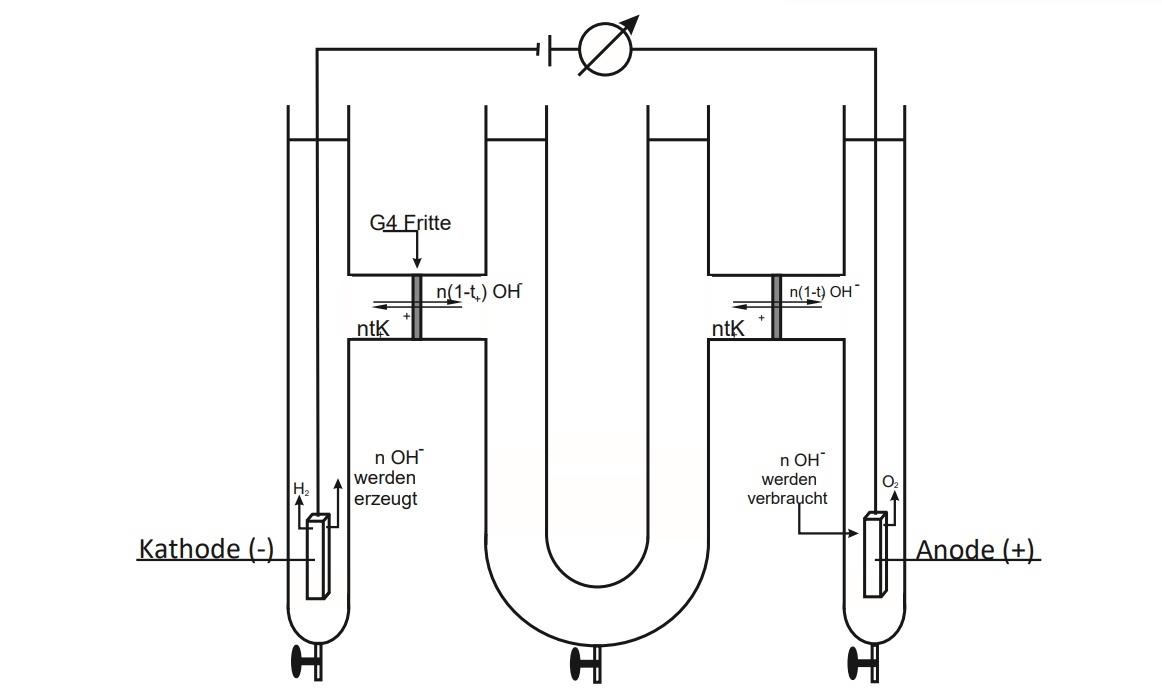
\includegraphics[scale=0.4]{Dreikammer.jpg}
\caption{Versuchsaufbau Teilversuch eins}
\end{figure}

Der Versuchteil 2 wurde nicht praktisch gemacht, Werte für den Versuchsteil 2 wurden uns bereitgestellt. 
Vor dem Versuch wurde Kontrolliert ob alle Geräte ausgeschaltet sind und auf 0 eingestellt sind, um Unfälle zu vermeiden da mit Gleichspannung gearbeitet wurde. Anschließend wurde der Pluspol des Spannungsgebers mit dem mA Eingang des Multimeters verbunden. Der COM Ausgang wurde mit der Anode des Elektrolysegefäßes Verbunden. Danach wurde die Kathode mit dem Minuspol des Spannungsgebers verbunden. Das untere Ende des U-Rohres ist über einem Stutzen mit Hahn mit einem Schlauch und einem Trichter verbunden. Die Vorbereitete Permanganat- Lösung wurde über einen Tropftrichter blasenfrei in den Schlauch gefüllt. Anschließend wurde der Hahn geöffnet um das gesamte Hahn-Volumen mit der Lösung zu fluten. Nach mehrmaligen ausspülen des U-Rohrs mit KNO$_{3}$-Lösung wurde das U-Rohr bis zur Hälfte der Schenkel befüllt. Danach werden die Elektroden eingehangen. Anschließend wurde der Hahn geöffnet um die KNO$_3$-Lösung mit der KMnO$_4$-Lösung zu unterschichten. Für eine scharfe Phasengrenzenausbildung werden die ersten cm innerhalb von einigen Minuten eingführt, dannach schneller. Die Elektrolyse wurde gestartet sobald die Elektroden ganz in der KNO$_3$-Lösung eingetaucht sind, und der Hahn geschlossen wurde. Die Elektrolyse dauert 20\ min bei 80\ v , dabei wurde alle 5\ min der Strom Protokoliert und die Position der Phasengrenzen an beiden Schenkel des U-Rohres markiert. 

\begin{figure}[H]
\centering
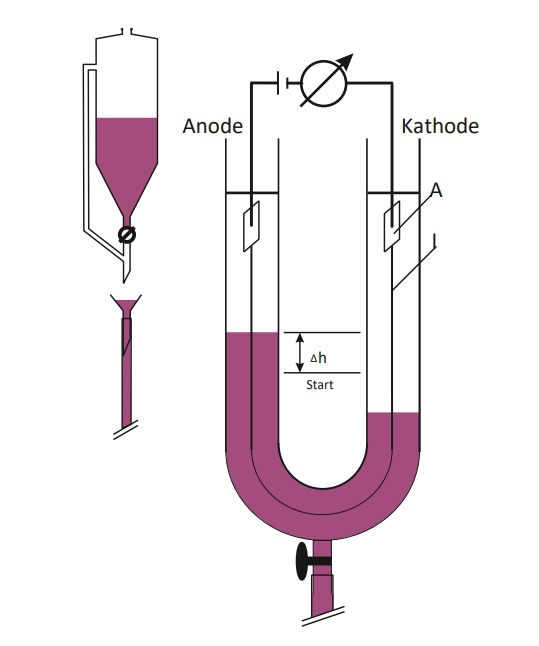
\includegraphics[scale=0.5]{Zweikammer.jpg}
\caption{Versuchsaufbau von Teilversuch zwei}
\end{figure}
